\documentclass[10pt,a4paper,titlepage]{article}
\usepackage{latexsym}
\usepackage[a4paper,top=2.5cm,bottom=2.5cm,left=2.5cm,right=2.5cm]{geometry}
\usepackage[utf8x]{inputenc}
\usepackage{booktabs,caption,amsfonts,amssymb,fancyhdr, amsmath}
\usepackage[english]{babel}
\usepackage{indentfirst}
\usepackage{float}
\renewcommand*{\familydefault}{\sfdefault}
\usepackage{graphicx}
\usepackage{hyperref}
\usepackage{color}
\usepackage{subcaption}
\usepackage{listings}

\lstset{language=c++}
\lstset{backgroundcolor=\color{white}}
\lstset{frame=single}
\lstset{stringstyle=\ttfamily}
\lstset{keywordstyle=\color{red}\bfseries}
\lstset{commentstyle=\itshape\color{blue}}

\captionsetup[table]{position=top}
\addtolength{\textwidth}{1cm}
\addtolength{\hoffset}{-1cm}
\pagestyle{headings}
\begin{document}
\begin{center}
{\LARGE \bfseries Computational Physics\par}
\vspace{0.5cm}
{\LARGE \bfseries Project 1 \par}
\end{center}

\vspace{1cm}

\begin{tabular*}{\textwidth}{@{}l@{\extracolsep{\fill}}l@{}}
Academic year 2015-2016	 &Team group: \\
						&Alessio Pizzini\\
                        & Giulio Isacchini\\
                        &Giovanni Pederiva\\
                      &Mattia Alberto Ubertini\\
                       
 
                        
\end{tabular*}
\begin{center}
\hrule height 2 pt
\end{center} 
\subsection*{Abstract}
The task for this project is to numerically solve a second order differential equation with a general pre-made algorithm and one specifically designed by us, in order to compare the results and the efficiency. We also made: an error analysis to determine if by decreasing the step length of the numerical algorithm some machine errors appeared; a time analysis, to count the number of FLOPS needed for the program to run and verify its efficiency.

\subsection*{Analysis of the problem}
In this project we've solved a one-dimensional Poisson equation with Dirichlet boundary conditions.
The equation reads: $-u^{''}(x)=f(x)$ with $x [0;1]$ and $u(0)=u(1)=0$.
These kinds of equations can be solved analytically. 
In our case, $f(x)=100e^{-10x}$, so that the previous equation has a solution 
$u_e(x)=1 − (1 − e^{−10} )x − e^ {−10x}$.
In this work we've solved it numerically and then we've compared our solution with the analytic one. \\
The first step we did has been the discretization of our domain and consequently of the functions in the equation. Then through the 3-point formula for the second derivative we've rewritten the equation in this way: $-\frac{u_{i-1}+u_{i+1}-2u_{i}}{h^2}=f_i$.
At this point the problem becomes a linear equation system with unknown variables the $u_{i}$, where $u_{i}$ means the function u evaluated at the point $x_{i}$ and the same with $f_{i}$.
The system can be written as $A u = \tilde {f}$ where  $\tilde {f}= h^2 f$. 
The matrix is tridiagonal, and the tridiagonal system related to it can be written as: $$a_iu_{i-1}+b_iu_i+c_iu_{i-1}=\tilde{f_i}$$
in our case the coefficients are constant, precisely $b=2$ , $ a=c=-1$. 
We've coded an algorithm for solving this system. 
The algorithm written is built upon the Gaussian elimination method and it consists in a procedure divided in two parts, the first step basically let us to reduce the matrix and consecutively to compute directly the last component $u_i$, in the second part we use the last component to compute recursively the previous ones. \\
We then solved the same problem without considering the simplification of the tridiagonal matrix, but using a brute force generic method like the LU decomposition, which is obviously more time consuming.


\subsection*{Tridiagonal Solver}
In order to solve the differential equation:
\[
-u''(x) = f(x), \hspace{0.5cm} x\in(0,1), \hspace{0.5cm} u(0) = u(1) = 0.
\]
we discretized the problem into the numerical equation
\[
   -\frac{u_{i+1}+u_{i-1}-2u_i}{h^2} = f_i  \hspace{0.5cm} \mathrm{for} \hspace{0.1cm} i=1,\dots, n,
\]
where $f_i=f(x_i)$.
If you define the three quantities:
\[
    {\bf A} = \left(\begin{array}{cccccc}
                           2& -1& 0 &\dots   & \dots &0 \\
                           -1 & 2 & -1 &0 &\dots &\dots \\
                           0&-1 &2 & -1 & 0 & \dots \\
                           0& \dots   & \dots &\dots   &\dots & \dots \\
                           0&\dots   &  &-1 &2& -1 \\
                           0&\dots    &  & 0  &-1 & 2 \\
                      \end{array} \right)
	\hspace{0.5cm}
    {\bf v} = \left(\begin{array}{c}
                           u_1\\
                           u_2\\
                           \dots\\
                           u_i\\
                           \dots\\
                           u_n\\
                      \end{array} \right)
                      \hspace{0.5cm}
	{\bf d} = \left(\begin{array}{c}
                           d_1\\
                           d_2\\
                           \dots\\
                           d_i\\
                           \dots\\
                           d_n\\
                      \end{array} \right)                  
\]
with $d_i=h^2 f_i$
it is trivial to show that the numerical equation can be rewritten as:
\[
   {\bf A}{\bf u} = {\bf d},
\]

\paragraph{General Tridiagonal Matrix Algorithm} Given a general tridiagonal matrix system:
\[
    {\bf M} = \left(\begin{array}{cccccc}
                           b_1& c_1& 0 &\dots   & \dots &0 \\
                           a_2 & b_2 & c_3 &0 &\dots &\dots \\
                           0&a_3 & b_3 & c_3 & 0 & \dots \\
                           0& \dots   & \dots &\dots   &\dots & 0 \\
                           0&\dots   &\dots  &\dots  &\dots& c_{n-1} \\
                           0&\dots &\dots  &0  &a_{n} & b_n \\
                      \end{array} \right)
                       \left(\begin{array}{c}
                           u_1\\
                           u_2\\
                           \dots\\
                           u_i\\
                           \dots\\
                           u_n\\
                      \end{array} \right)
	= \left(\begin{array}{c}
                           d_1\\
                           d_2\\
                           \dots\\
                           d_i\\
                           \dots\\
                           d_n\\
                      \end{array} \right)    
\]   
The algorithm can be summed up in\footnote{The apex x' represents a variable that has been modified in the previous step}:
\begin{itemize} 
\item Forward substitution:
\[
	a'_i = 0 \hspace{0.3cm} i = 2, \dots, n \hspace{0.8cm} 
    b'_i = \begin{cases} 
			b_i  & i=1 \\
			b_i - \frac{a_i c_i}{ b'_{i-1}} & i=2,\dots,n 
		\end{cases}
\]

\[
	c'_i = c_i \hspace{0.3cm} i = 1, \dots, n \hspace{0.9cm} 
	d'_i= \begin{cases} 
					d_i  & i=1 \\
					d_i - \frac{a_i d'_{i-1}}{b'_{i-1}} & i=2,\dots,n
				\end{cases}
\]

\item Backward substitution:
\[
	u_i = \begin{cases} 
			d'_i  & i = n \\
			\frac{d'_i + u_{i+1} c'_i}{b_i} & i=n-1,n-2,\dots,1 
		\end{cases}
\]
\end{itemize}

We can easily count that the total amount of FLOPS used for each step is equal to 9, so this algorithm is of class $O(9n)$. This is much faster than the two standard methods of Gaussian elimination and LU decomposition which both are of class $O(n^3)$.
\paragraph{Further simplification}
By looking at the previous equation and considering the nature of the coefficients $a_i,b_i,c_i$ we can reduce the number of FLOPS to 6 for each step.
The equations now read:
\[
	b'_i= \begin{cases} 
					b_i  & i=1 \\
					b_i - \frac{1}{b'_{i-1}} & i=2,\dots,n
				\end{cases}	
                \hspace{0.9cm} 
	d'_i= \begin{cases} 
					d_i  & i=1 \\
					d_i + \frac{d'_{i-1}}{b'_{i-1}} & i=2,\dots,n
				\end{cases}
\] for the forward substitution, and 
\[
	u_i = \begin{cases} 
			\frac{d'_i}{b'_i}   & i = n \\
			\frac{d'_i - u_{i+1} }{b_i} & i=n-1,n-2,\dots,1 
		\end{cases}
\] for the backward substitution. We now have an algorithm that is of order $O(6n)$ 

\subsection*{Implementation}
We wrote a $C++$ code to solve this problem\footnote{The full code is at the ending of the paper or on GitHub \url{https://github.com/GioPede/FYS3150/blob/master/Project1/prj1/main.cpp}} and developed a function that returns a vector that is the discrete solution of the differential equation. 

\begin{lstlisting}[title={Solve Tridiagonal Matrix}]

//Fuction to compute the solution of the differential equation
//using the gaussian elimination on the tridiagonal matrix
//      - u''(x) + f(x) = 0
double * compute_vectors (unsigned int size, //the size of the arrays
                          double *A,         //the lower diagonal coefficients 
                          double *B,         //the main diagonal coefficients 
                          double *C,         //the upper diagonal coefficients 
                          double *D,         //the source terms f(x_i)*h^2
                          bool speed = 0)    //a boolean whether the function 
                                             //should run with the simplified 
                                             //6n algorithm
{
	double *U = new double[size]; //the solution vector
	
	//General tridiagonal matrix solver
	if(!speed){
		//forward substitution
		for (unsigned int i = 1; i < size; i++){
			B[i] = B[i] - A[i] / B[i - 1] * C[i];
			D[i] = D[i] - D[i - 1] * A[i] / B[i - 1];
		}
		//backward substitution
		v[size - 1] = D[size - 1];
		for (int i = size - 2; i >= 0; i--)
			U[i] = (D[i] -  C[i] * U[i + 1] ) / B[i];
	}
	
	
	//Optimized 6n algorithm for the particular problem
	else {
		//forward substitution
		for (unsigned int i = 1; i < size; i++){
			B[i] -= 1 / B[i - 1];
			D[i] += D[i - 1] / B[i - 1];
		}	
		//backward substitution
		v[size - 1] = D[size - 1] / B[size - 1];
		for (int i = size - 2; i >= 0; i--)
			U[i] = (D[i] + U[i + 1]) / B[i];
	}	
	return U;
	delete [] U;
}

\end{lstlisting}

We then used this function for different sizes of vectors, going from $10$ to $10^6$, to which corresponded the step lengths going from $h = 10^{-1}$ to $h = 10^{-6}$.

Afterwards an LU decomposition solver was developed, using some pre-made functions. This solver only takes as arguments the matrix {\bf A} and the source terms vector {\bf v} . 

\begin{lstlisting}[title={Solve LU decomposition}]
double * compute_matrix (unsigned int size, //the size of the arrays
                         double **A,        //the matrix of coefficients
                         double *B)         //the source terms vector
{
	int *indx = new int[size];
	double d;
    
	ludcmp(A, size, indx, &d);  //decompose the matrix
	lubksb(A, size, indx, B);   //backward substitution to solve the linear system
    
	delete [] indx;
	return B;
}
\end{lstlisting}

This last method couldn't be run for small values of $h$, we could only get to $10^{-3}$ because the memory needed to store the matrix increases as the $n^2$, with $n$ the size, and we would have finished the RAM of our laptops with already $h= 10^{-5}$ (this would have taken 10 GB of memory). \\
But this is not the main problem that arises. The number of FLOPS of this algorithm scales as $O(n^3)$ like the standard Gaussian elimination, so the time of computation scales in the same way. A step length of $10^{-4}$ would have required around 40 minutes of time.

\subsection*{Analysis of the results}
\paragraph{Solution plots analysis}
To analyze the results, we plotted the different solutions we found with different values of $h$ together with the analytical solution versus the variable x: \\
\begin{minipage}{0.6\textwidth}
	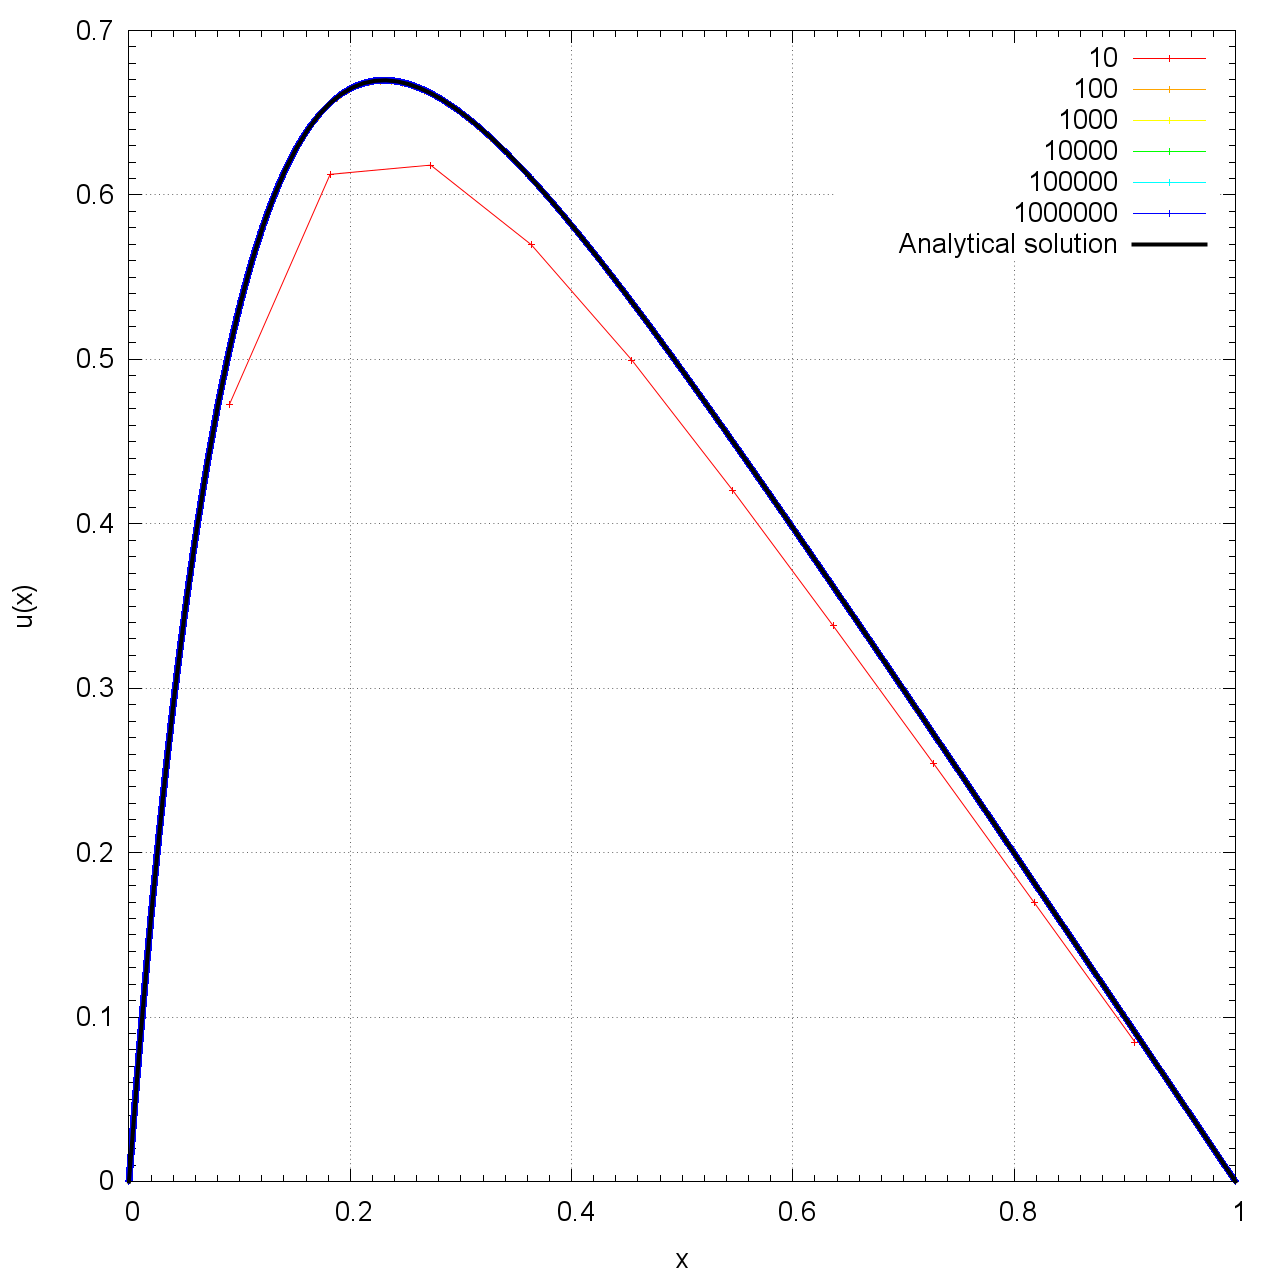
\includegraphics[width=0.8\columnwidth]{plot.png}
    \captionof{figure}{{\footnotesize  Gaussian elimination derived algorithm's plot of the\\ computed solutions}}
\end{minipage}
\begin{minipage}{0.6\textwidth}
	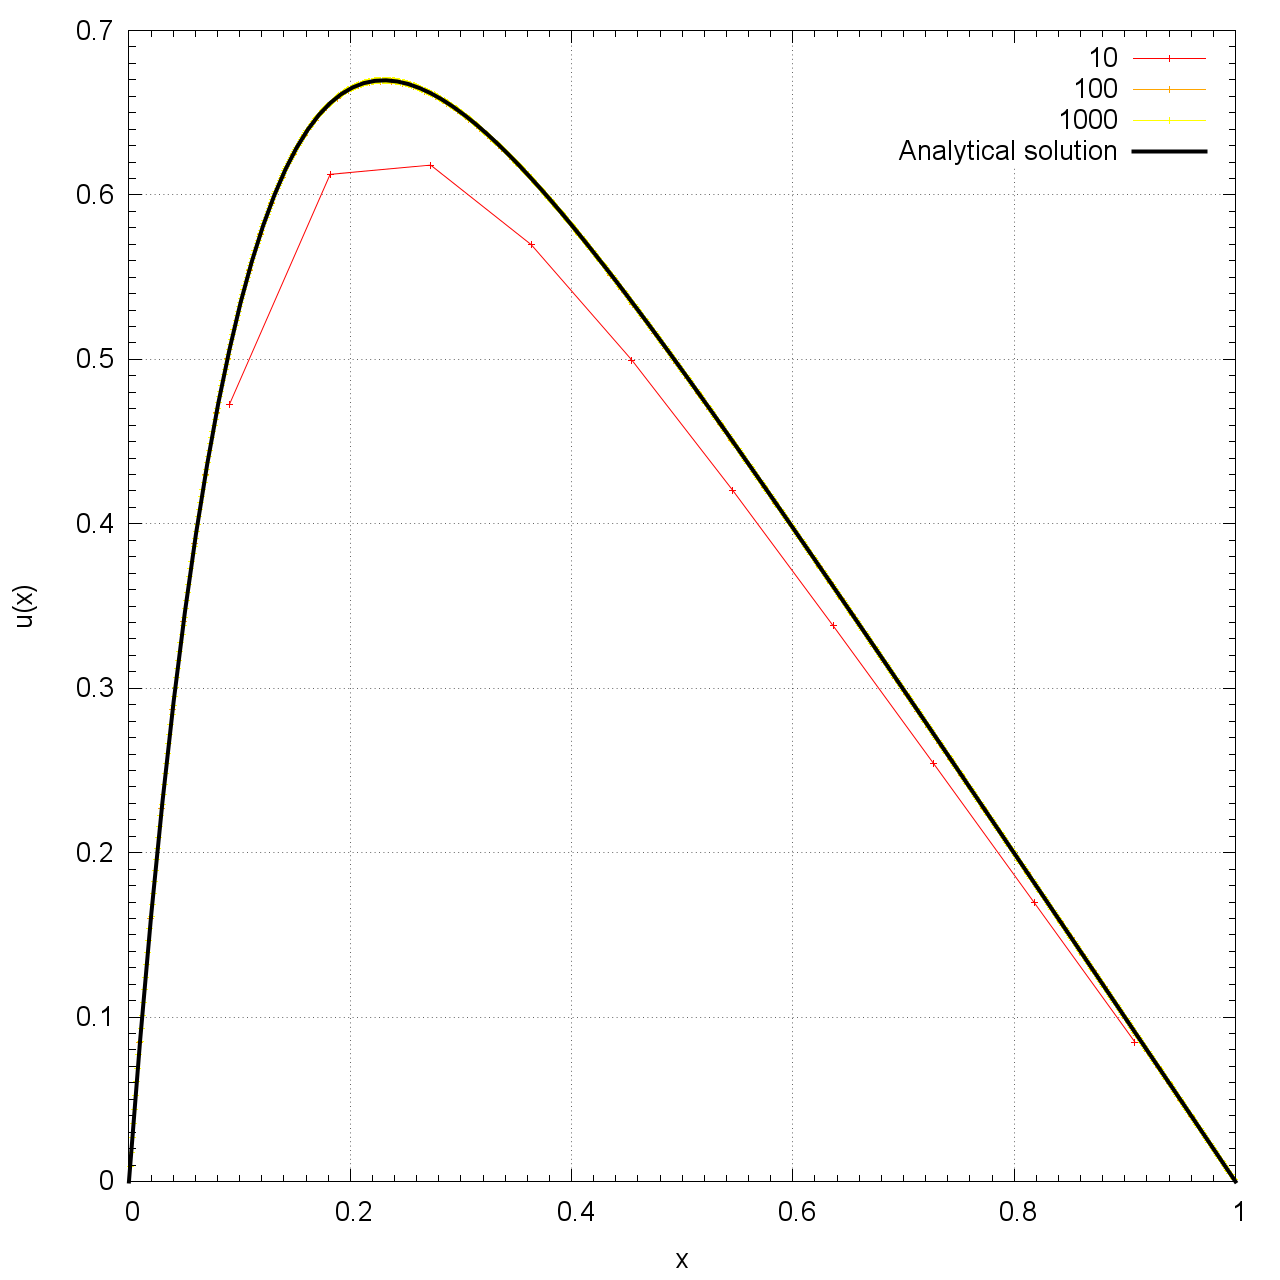
\includegraphics[width=0.8\textwidth]{plotLU.png}
    \captionof{figure}{{\footnotesize  LU decomposition derived algorithm's plot of the\\ computed solutions}}
\end{minipage}\\

We can immediately see that the two different methods that we've used give more or less the same output in terms of convergence, the 10 points series is far from the analytical solution, but the others are very good approximations. Moreover we can see that the two methods are equivalent for the 10 points plot, and they are for all data series in fact, they are equivalent.\\

\paragraph{Error analysis}
Apart from the solution obtained with only 10 points, every other solution we found with the tridiagonal algorithm looks identical to the analytical one.
To get a closer look to the precision of our algorithm we plotted a graph showing the relative error of the approximated solution in respect to the analytical one (on a logarithmic scale) versus the variable x for each value of the step lenght $h$ we computed:
\begin{center}
	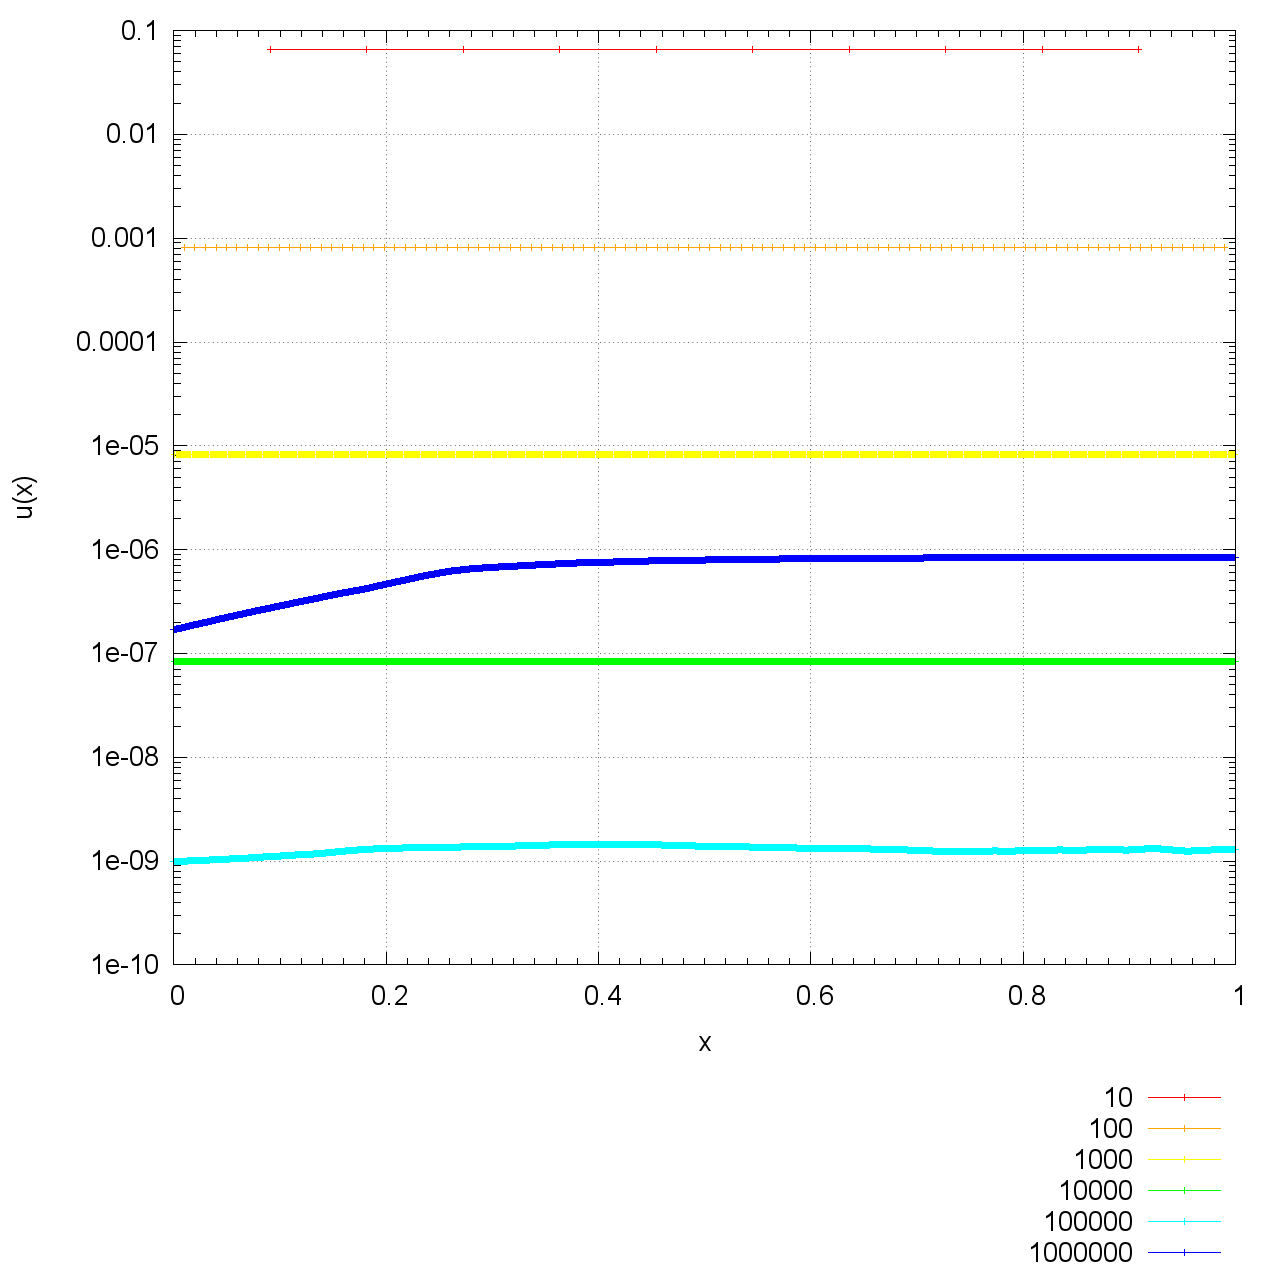
\includegraphics[width=0.5\columnwidth]{plot_err.png}		\captionof{figure}{{\footnotesize Relative error as a function of position for all the data series of the tridiagonal algorithm }}
\end{center}
    As for the five highest values of $h$ (i.e. for the lowest numbers of points computed), the error decreases as $\frac{1}{h^2}$ for the whole interval of x, as expected since the second derivative approximation we are using has a convergence rate of $\frac{1}{h^2}$. As for the lowest value of $h$, our extimate of the function gets worse. This should happen due to loss of numerical precision of the machine, which appears when we are subtracting two almost identical numbers, as it happens when we are evaluating a function in two points very next to each other.
To understand better how the precision of our algorithm depends on the step length $h$, we plotted a graph showing the modulus of the difference between our extimate of the value of the function for x=0.5 and the value of the analytical value for the same value of x versus the step lenght $h$:
\begin{center}
	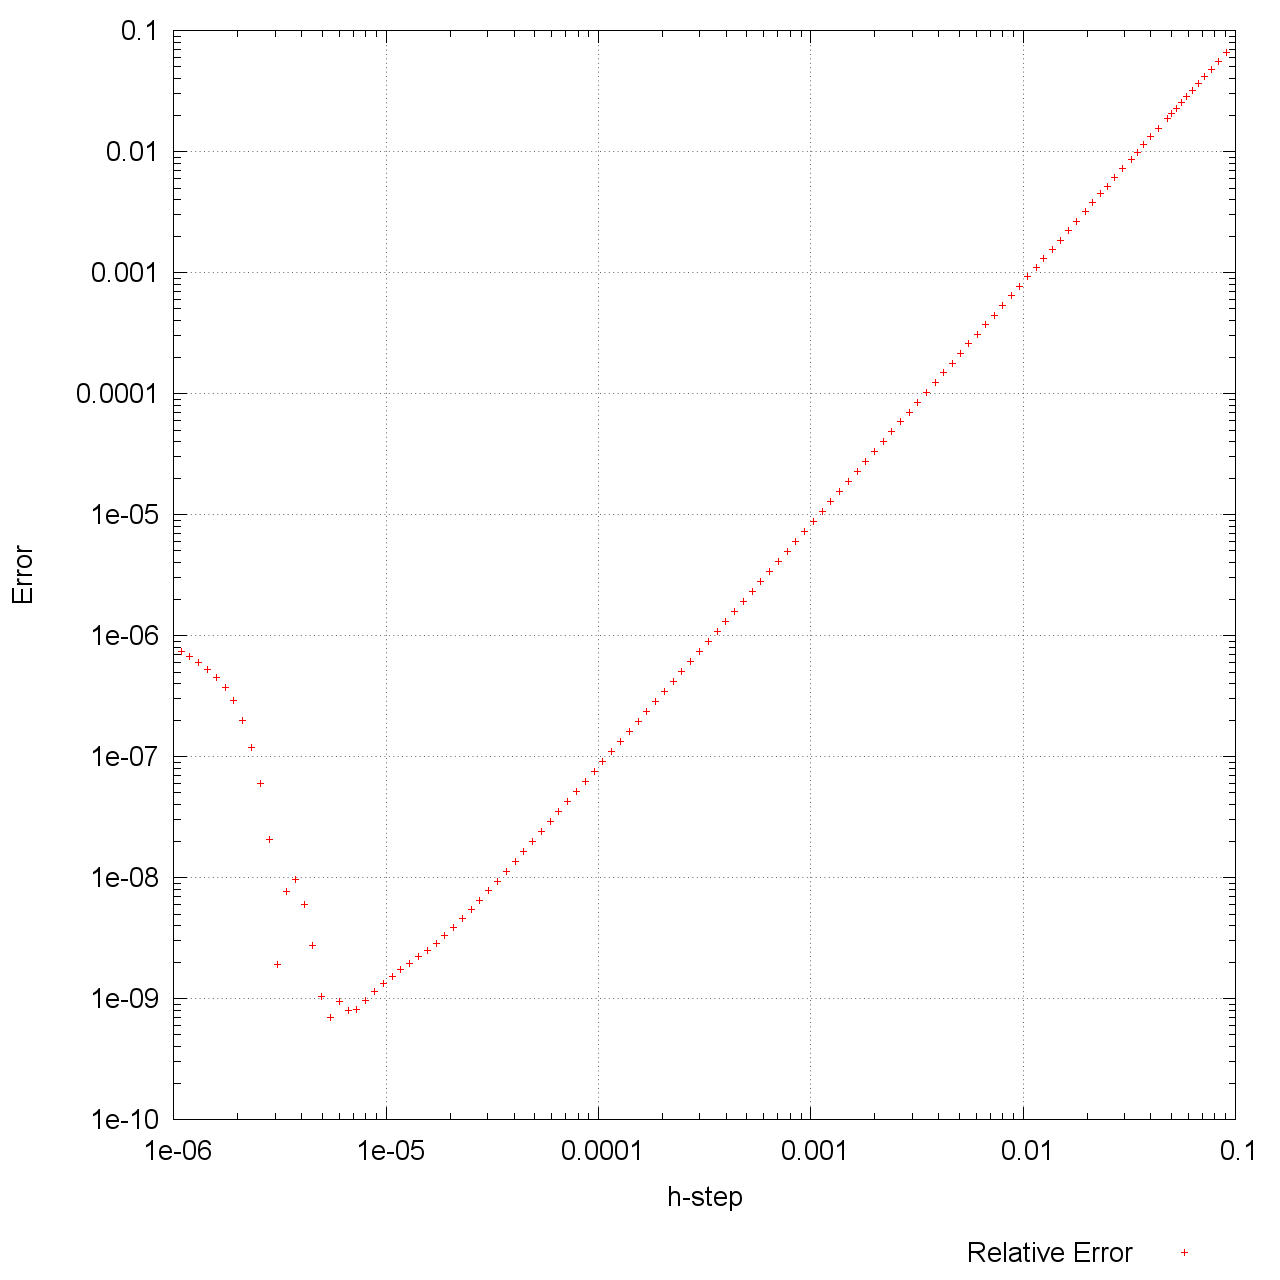
\includegraphics[width=0.5\columnwidth]{error.png}
\end{center}
It is now clear that there are two sources of error: the machine error, which is preponderant for smaller values of $h$, and the approximation error, preponderant for bigger values of h. It is possible to find the value of $h$ minimizing the total error simply by computing the derivative of the formula for the total error on the variable $h$: the three points formula error is given by: 
$$\varepsilon_{3p}=\frac{f^{(3)}*h^{2}}{6}$$
while the machine roundoff error is: 
$$\varepsilon_{m}=\frac{\varepsilon_{0}}{2*h}$$ 
The best choice for $h$ hence is 
$$\varepsilon_{min} = \sqrt[3]{\frac{3*\varepsilon_{0}}{2*f^{(3)}}}$$
Evaluating this formula in our case, and assuming $\varepsilon = 10^{-15}$ one gets $h\simeq1.2*10^{-5}$, which is close to the value we can extract from the previous graph.\\ 
An analogous analysis has been carried out for the LU decomposition, but we couldn't increase the number of points over 1000 since the number of FLOPS scales as $O_(n^{3})$ (while in our simplified version of the Gaussian elimination this number scales as $O(n)$). Here's the result:
\begin{center}
	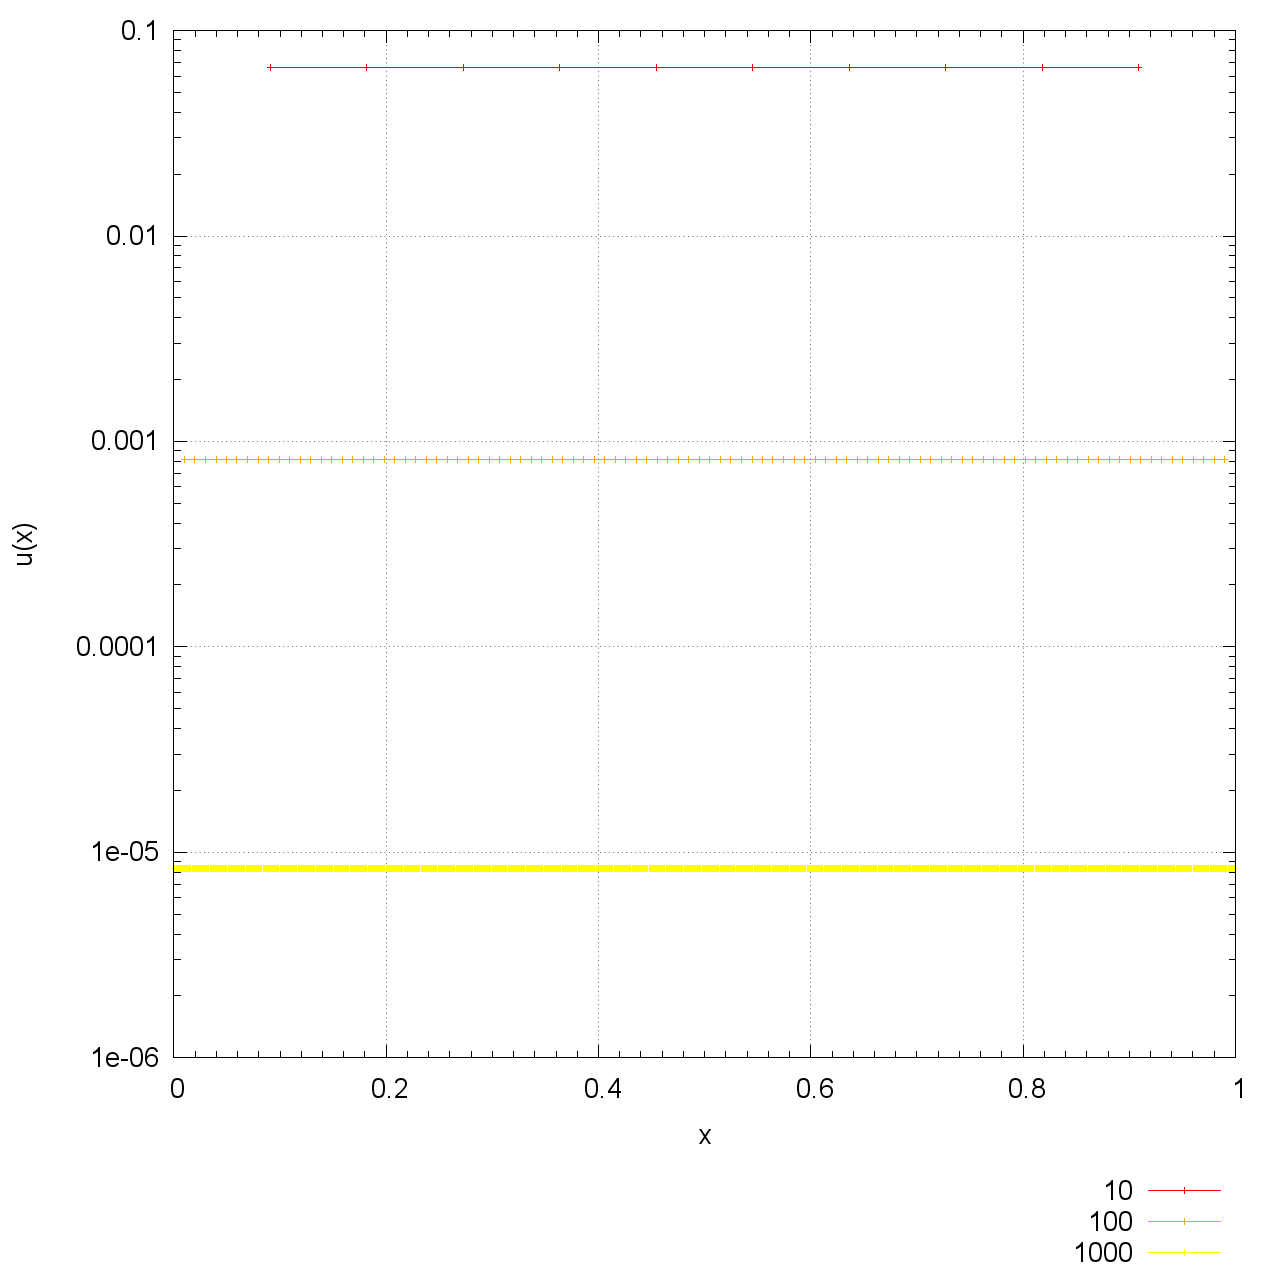
\includegraphics[width=0.5\columnwidth]{plot_errLU.png}
\end{center}
The error is the same as with the previous algorithms with equal step length $h$ and as in the previous case, the error scales as $\frac{1}{h^{2}}$. 
The influence of the roundoff error can't be seen since $h$ is never small enough. 

\paragraph{Elapsed time}
In the end, we analyzed how the elapsed time for the code to run depends on the algorithm and on the step length h. 
\begin{center}
\begin{tabular}{ |c|c|c|c| }
\hline
$h$ & Vector 9 FLOPS & Vector 6 FLOPS & Matrix \\\hline
  $10^{-1}$      & 0.000002 s& 0.000003 s& 0.000015 s \\\hline
  $10^{-2}$    & 0.000004 s& 0.000004 s& 0.001454 s \\\hline
  $10^{-3}$  & 0.000042 s& 0.000039 s& 1.896924 s \\\hline
  $10^{-4}$ & 0.000409 s& 0.000349 s& $/$\\\hline
  $10^{-5}$ & 0.004137 s& 0.003818 s& $/$\\\hline
  $10^{-6}$ & 0.046839 s& 0.038214 s& $/$\\\hline
\end{tabular}
\end{center}
As expected, the time elapsed scales about as $O(n)$ as for the simplified algorithm for tridiaginal matrices,  while is scales as $O(n^3)$ for the LU decomposition.  It's a little faster for the $O(6n)$ but not as much as we were expecting, probably because we are not considering other minor operations required for the algorithm (such as index operations) that reduce the rate between the two. \\
We can also notice that the values for $h = 0.1$ are higher than expected for all algorithms, this is probably due to the fact that the total number of operation is really limited, and the time elapsed for other CPU operations (like the call of the function itself) take an amount of time comparable to the one of the operations.

\subsection*{Conclusions}
We believe that this project has been really useful to understand both how to implement linear algebra calculations and how to solve differential equations numerically being aware of the problem that could arise. It would also have been interesting to test the algorithm with more irregular functions (more sloped ones, or functions which are non-differentiable in some points).\\
The simplified version of Gaussian elimination turned out to be equivalent in results to the LU decomposition, as we were expecting, but much more efficient than LU decomposition both in the amount of RAM memory required and in the time elapsed. For example, for $h=10^{-3}$, the 6 FLOPS vector algorithm is about 50.000 times faster than LU decomposition, so the former algorithm is to be preferred, especially when a big amount of calculations is needed.
Nevertheless, being in our case the x interval so short, it has been possible to find a numerical solution which relative error is lower than $10^{-5}$ with an elapsed times in the order of seconds even with plain LU decomposition.
\end{document}